%
\begin{isabellebody}%
\def\isabellecontext{Examples{\isadigit{3}}}%
%
\isadelimtheory
%
\endisadelimtheory
%
\isatagtheory
\isacommand{theory}\isamarkupfalse%
\ Examples{\isadigit{3}}\isanewline
\isakeyword{imports}\ Examples\isanewline
\isakeyword{begin}%
\endisatagtheory
{\isafoldtheory}%
%
\isadelimtheory
%
\endisadelimtheory
%
\begin{isamarkuptext}%
\vspace{-5ex}%
\end{isamarkuptext}%
\isamarkuptrue%
%
\isamarkupsubsection{Third Version: Local Interpretation
  \label{sec:local-interpretation}%
}
\isamarkuptrue%
%
\begin{isamarkuptext}%
In the above example, the fact that \isa{op\ {\isaliteral{5C3C6C653E}{\isasymle}}} is a partial
  order for the integers was used in the second goal to
  discharge the premise in the definition of \isa{op\ {\isaliteral{5C3C73717375627365743E}{\isasymsqsubset}}}.  In
  general, proofs of the equations not only may involve definitions
  from the interpreted locale but arbitrarily complex arguments in the
  context of the locale.  Therefore it would be convenient to have the
  interpreted locale conclusions temporarily available in the proof.
  This can be achieved by a locale interpretation in the proof body.
  The command for local interpretations is \isakeyword{interpret}.  We
  repeat the example from the previous section to illustrate this.%
\end{isamarkuptext}%
\isamarkuptrue%
%
\isadelimvisible
\ \ %
\endisadelimvisible
%
\isatagvisible
\isacommand{interpretation}\isamarkupfalse%
\ int{\isaliteral{3A}{\isacharcolon}}\ partial{\isaliteral{5F}{\isacharunderscore}}order\ {\isaliteral{22}{\isachardoublequoteopen}}op\ {\isaliteral{5C3C6C653E}{\isasymle}}\ {\isaliteral{3A}{\isacharcolon}}{\isaliteral{3A}{\isacharcolon}}\ int\ {\isaliteral{5C3C52696768746172726F773E}{\isasymRightarrow}}\ int\ {\isaliteral{5C3C52696768746172726F773E}{\isasymRightarrow}}\ bool{\isaliteral{22}{\isachardoublequoteclose}}\isanewline
\ \ \ \ \isakeyword{where}\ {\isaliteral{22}{\isachardoublequoteopen}}int{\isaliteral{2E}{\isachardot}}less\ x\ y\ {\isaliteral{3D}{\isacharequal}}\ {\isaliteral{28}{\isacharparenleft}}x\ {\isaliteral{3C}{\isacharless}}\ y{\isaliteral{29}{\isacharparenright}}{\isaliteral{22}{\isachardoublequoteclose}}\isanewline
\ \ \isacommand{proof}\isamarkupfalse%
\ {\isaliteral{2D}{\isacharminus}}\isanewline
\ \ \ \ \isacommand{show}\isamarkupfalse%
\ {\isaliteral{22}{\isachardoublequoteopen}}partial{\isaliteral{5F}{\isacharunderscore}}order\ {\isaliteral{28}{\isacharparenleft}}op\ {\isaliteral{5C3C6C653E}{\isasymle}}\ {\isaliteral{3A}{\isacharcolon}}{\isaliteral{3A}{\isacharcolon}}\ int\ {\isaliteral{5C3C52696768746172726F773E}{\isasymRightarrow}}\ int\ {\isaliteral{5C3C52696768746172726F773E}{\isasymRightarrow}}\ bool{\isaliteral{29}{\isacharparenright}}{\isaliteral{22}{\isachardoublequoteclose}}\isanewline
\ \ \ \ \ \ \isacommand{by}\isamarkupfalse%
\ unfold{\isaliteral{5F}{\isacharunderscore}}locales\ auto\isanewline
\ \ \ \ \isacommand{then}\isamarkupfalse%
\ \isacommand{interpret}\isamarkupfalse%
\ int{\isaliteral{3A}{\isacharcolon}}\ partial{\isaliteral{5F}{\isacharunderscore}}order\ {\isaliteral{22}{\isachardoublequoteopen}}op\ {\isaliteral{5C3C6C653E}{\isasymle}}\ {\isaliteral{3A}{\isacharcolon}}{\isaliteral{3A}{\isacharcolon}}\ {\isaliteral{5B}{\isacharbrackleft}}int{\isaliteral{2C}{\isacharcomma}}\ int{\isaliteral{5D}{\isacharbrackright}}\ {\isaliteral{5C3C52696768746172726F773E}{\isasymRightarrow}}\ bool{\isaliteral{22}{\isachardoublequoteclose}}\ \isacommand{{\isaliteral{2E}{\isachardot}}}\isamarkupfalse%
\isanewline
\ \ \ \ \isacommand{show}\isamarkupfalse%
\ {\isaliteral{22}{\isachardoublequoteopen}}int{\isaliteral{2E}{\isachardot}}less\ x\ y\ {\isaliteral{3D}{\isacharequal}}\ {\isaliteral{28}{\isacharparenleft}}x\ {\isaliteral{3C}{\isacharless}}\ y{\isaliteral{29}{\isacharparenright}}{\isaliteral{22}{\isachardoublequoteclose}}\isanewline
\ \ \ \ \ \ \isacommand{unfolding}\isamarkupfalse%
\ int{\isaliteral{2E}{\isachardot}}less{\isaliteral{5F}{\isacharunderscore}}def\ \isacommand{by}\isamarkupfalse%
\ auto\isanewline
\ \ \isacommand{qed}\isamarkupfalse%
%
\endisatagvisible
{\isafoldvisible}%
%
\isadelimvisible
%
\endisadelimvisible
%
\begin{isamarkuptext}%
The inner interpretation is immediate from the preceding fact
  and proved by assumption (Isar short hand ``.'').  It enriches the
  local proof context by the theorems
  also obtained in the interpretation from Section~\ref{sec:po-first},
  and \isa{int{\isaliteral{2E}{\isachardot}}less{\isaliteral{5F}{\isacharunderscore}}def} may directly be used to unfold the
  definition.  Theorems from the local interpretation disappear after
  leaving the proof context --- that is, after the succeeding
  \isakeyword{next} or \isakeyword{qed} statement.%
\end{isamarkuptext}%
\isamarkuptrue%
%
\isamarkupsubsection{Further Interpretations%
}
\isamarkuptrue%
%
\begin{isamarkuptext}%
Further interpretations are necessary for
  the other locales.  In \isa{lattice} the operations~\isa{{\isaliteral{5C3C7371696E7465723E}{\isasymsqinter}}}
  and~\isa{{\isaliteral{5C3C7371756E696F6E3E}{\isasymsqunion}}} are substituted by \isa{min}
  and \isa{max}.  The entire proof for the
  interpretation is reproduced to give an example of a more
  elaborate interpretation proof.  Note that the equations are named
  so they can be used in a later example.%
\end{isamarkuptext}%
\isamarkuptrue%
%
\isadelimvisible
\ \ %
\endisadelimvisible
%
\isatagvisible
\isacommand{interpretation}\isamarkupfalse%
\ int{\isaliteral{3A}{\isacharcolon}}\ lattice\ {\isaliteral{22}{\isachardoublequoteopen}}op\ {\isaliteral{5C3C6C653E}{\isasymle}}\ {\isaliteral{3A}{\isacharcolon}}{\isaliteral{3A}{\isacharcolon}}\ int\ {\isaliteral{5C3C52696768746172726F773E}{\isasymRightarrow}}\ int\ {\isaliteral{5C3C52696768746172726F773E}{\isasymRightarrow}}\ bool{\isaliteral{22}{\isachardoublequoteclose}}\isanewline
\ \ \ \ \isakeyword{where}\ int{\isaliteral{5F}{\isacharunderscore}}min{\isaliteral{5F}{\isacharunderscore}}eq{\isaliteral{3A}{\isacharcolon}}\ {\isaliteral{22}{\isachardoublequoteopen}}int{\isaliteral{2E}{\isachardot}}meet\ x\ y\ {\isaliteral{3D}{\isacharequal}}\ min\ x\ y{\isaliteral{22}{\isachardoublequoteclose}}\isanewline
\ \ \ \ \ \ \isakeyword{and}\ int{\isaliteral{5F}{\isacharunderscore}}max{\isaliteral{5F}{\isacharunderscore}}eq{\isaliteral{3A}{\isacharcolon}}\ {\isaliteral{22}{\isachardoublequoteopen}}int{\isaliteral{2E}{\isachardot}}join\ x\ y\ {\isaliteral{3D}{\isacharequal}}\ max\ x\ y{\isaliteral{22}{\isachardoublequoteclose}}\isanewline
\ \ \isacommand{proof}\isamarkupfalse%
\ {\isaliteral{2D}{\isacharminus}}\isanewline
\ \ \ \ \isacommand{show}\isamarkupfalse%
\ {\isaliteral{22}{\isachardoublequoteopen}}lattice\ {\isaliteral{28}{\isacharparenleft}}op\ {\isaliteral{5C3C6C653E}{\isasymle}}\ {\isaliteral{3A}{\isacharcolon}}{\isaliteral{3A}{\isacharcolon}}\ int\ {\isaliteral{5C3C52696768746172726F773E}{\isasymRightarrow}}\ int\ {\isaliteral{5C3C52696768746172726F773E}{\isasymRightarrow}}\ bool{\isaliteral{29}{\isacharparenright}}{\isaliteral{22}{\isachardoublequoteclose}}%
\begin{isamarkuptxt}%
\normalsize We have already shown that this is a partial
        order,%
\end{isamarkuptxt}%
\isamarkuptrue%
\ \ \ \ \ \ \isacommand{apply}\isamarkupfalse%
\ unfold{\isaliteral{5F}{\isacharunderscore}}locales%
\begin{isamarkuptxt}%
\normalsize hence only the lattice axioms remain to be
        shown.
        \begin{isabelle}%
\ {\isadigit{1}}{\isaliteral{2E}{\isachardot}}\ {\isaliteral{5C3C416E643E}{\isasymAnd}}x\ y{\isaliteral{2E}{\isachardot}}\ {\isaliteral{5C3C6578697374733E}{\isasymexists}}inf{\isaliteral{2E}{\isachardot}}\ partial{\isaliteral{5F}{\isacharunderscore}}order{\isaliteral{2E}{\isachardot}}is{\isaliteral{5F}{\isacharunderscore}}inf\ op\ {\isaliteral{5C3C6C653E}{\isasymle}}\ x\ y\ inf\isanewline
\ {\isadigit{2}}{\isaliteral{2E}{\isachardot}}\ {\isaliteral{5C3C416E643E}{\isasymAnd}}x\ y{\isaliteral{2E}{\isachardot}}\ {\isaliteral{5C3C6578697374733E}{\isasymexists}}sup{\isaliteral{2E}{\isachardot}}\ partial{\isaliteral{5F}{\isacharunderscore}}order{\isaliteral{2E}{\isachardot}}is{\isaliteral{5F}{\isacharunderscore}}sup\ op\ {\isaliteral{5C3C6C653E}{\isasymle}}\ x\ y\ sup%
\end{isabelle}
        By \isa{is{\isaliteral{5F}{\isacharunderscore}}inf} and \isa{is{\isaliteral{5F}{\isacharunderscore}}sup},%
\end{isamarkuptxt}%
\isamarkuptrue%
\ \ \ \ \ \ \isacommand{apply}\isamarkupfalse%
\ {\isaliteral{28}{\isacharparenleft}}unfold\ int{\isaliteral{2E}{\isachardot}}is{\isaliteral{5F}{\isacharunderscore}}inf{\isaliteral{5F}{\isacharunderscore}}def\ int{\isaliteral{2E}{\isachardot}}is{\isaliteral{5F}{\isacharunderscore}}sup{\isaliteral{5F}{\isacharunderscore}}def{\isaliteral{29}{\isacharparenright}}%
\begin{isamarkuptxt}%
\normalsize the goals are transformed to these
        statements:
        \begin{isabelle}%
\ {\isadigit{1}}{\isaliteral{2E}{\isachardot}}\ {\isaliteral{5C3C416E643E}{\isasymAnd}}x\ y{\isaliteral{2E}{\isachardot}}\ {\isaliteral{5C3C6578697374733E}{\isasymexists}}inf{\isaliteral{5C3C6C653E}{\isasymle}}x{\isaliteral{2E}{\isachardot}}\ inf\ {\isaliteral{5C3C6C653E}{\isasymle}}\ y\ {\isaliteral{5C3C616E643E}{\isasymand}}\ {\isaliteral{28}{\isacharparenleft}}{\isaliteral{5C3C666F72616C6C3E}{\isasymforall}}z{\isaliteral{2E}{\isachardot}}\ z\ {\isaliteral{5C3C6C653E}{\isasymle}}\ x\ {\isaliteral{5C3C616E643E}{\isasymand}}\ z\ {\isaliteral{5C3C6C653E}{\isasymle}}\ y\ {\isaliteral{5C3C6C6F6E6772696768746172726F773E}{\isasymlongrightarrow}}\ z\ {\isaliteral{5C3C6C653E}{\isasymle}}\ inf{\isaliteral{29}{\isacharparenright}}\isanewline
\ {\isadigit{2}}{\isaliteral{2E}{\isachardot}}\ {\isaliteral{5C3C416E643E}{\isasymAnd}}x\ y{\isaliteral{2E}{\isachardot}}\ {\isaliteral{5C3C6578697374733E}{\isasymexists}}sup{\isaliteral{5C3C67653E}{\isasymge}}x{\isaliteral{2E}{\isachardot}}\ y\ {\isaliteral{5C3C6C653E}{\isasymle}}\ sup\ {\isaliteral{5C3C616E643E}{\isasymand}}\ {\isaliteral{28}{\isacharparenleft}}{\isaliteral{5C3C666F72616C6C3E}{\isasymforall}}z{\isaliteral{2E}{\isachardot}}\ x\ {\isaliteral{5C3C6C653E}{\isasymle}}\ z\ {\isaliteral{5C3C616E643E}{\isasymand}}\ y\ {\isaliteral{5C3C6C653E}{\isasymle}}\ z\ {\isaliteral{5C3C6C6F6E6772696768746172726F773E}{\isasymlongrightarrow}}\ sup\ {\isaliteral{5C3C6C653E}{\isasymle}}\ z{\isaliteral{29}{\isacharparenright}}%
\end{isabelle}
        This is Presburger arithmetic, which can be solved by the
        method \isa{arith}.%
\end{isamarkuptxt}%
\isamarkuptrue%
\ \ \ \ \ \ \isacommand{by}\isamarkupfalse%
\ arith{\isaliteral{2B}{\isacharplus}}%
\begin{isamarkuptxt}%
\normalsize In order to show the equations, we put ourselves
      in a situation where the lattice theorems can be used in a
      convenient way.%
\end{isamarkuptxt}%
\isamarkuptrue%
\ \ \ \ \isacommand{then}\isamarkupfalse%
\ \isacommand{interpret}\isamarkupfalse%
\ int{\isaliteral{3A}{\isacharcolon}}\ lattice\ {\isaliteral{22}{\isachardoublequoteopen}}op\ {\isaliteral{5C3C6C653E}{\isasymle}}\ {\isaliteral{3A}{\isacharcolon}}{\isaliteral{3A}{\isacharcolon}}\ int\ {\isaliteral{5C3C52696768746172726F773E}{\isasymRightarrow}}\ int\ {\isaliteral{5C3C52696768746172726F773E}{\isasymRightarrow}}\ bool{\isaliteral{22}{\isachardoublequoteclose}}\ \isacommand{{\isaliteral{2E}{\isachardot}}}\isamarkupfalse%
\isanewline
\ \ \ \ \isacommand{show}\isamarkupfalse%
\ {\isaliteral{22}{\isachardoublequoteopen}}int{\isaliteral{2E}{\isachardot}}meet\ x\ y\ {\isaliteral{3D}{\isacharequal}}\ min\ x\ y{\isaliteral{22}{\isachardoublequoteclose}}\isanewline
\ \ \ \ \ \ \isacommand{by}\isamarkupfalse%
\ {\isaliteral{28}{\isacharparenleft}}bestsimp\ simp{\isaliteral{3A}{\isacharcolon}}\ int{\isaliteral{2E}{\isachardot}}meet{\isaliteral{5F}{\isacharunderscore}}def\ int{\isaliteral{2E}{\isachardot}}is{\isaliteral{5F}{\isacharunderscore}}inf{\isaliteral{5F}{\isacharunderscore}}def{\isaliteral{29}{\isacharparenright}}\isanewline
\ \ \ \ \isacommand{show}\isamarkupfalse%
\ {\isaliteral{22}{\isachardoublequoteopen}}int{\isaliteral{2E}{\isachardot}}join\ x\ y\ {\isaliteral{3D}{\isacharequal}}\ max\ x\ y{\isaliteral{22}{\isachardoublequoteclose}}\isanewline
\ \ \ \ \ \ \isacommand{by}\isamarkupfalse%
\ {\isaliteral{28}{\isacharparenleft}}bestsimp\ simp{\isaliteral{3A}{\isacharcolon}}\ int{\isaliteral{2E}{\isachardot}}join{\isaliteral{5F}{\isacharunderscore}}def\ int{\isaliteral{2E}{\isachardot}}is{\isaliteral{5F}{\isacharunderscore}}sup{\isaliteral{5F}{\isacharunderscore}}def{\isaliteral{29}{\isacharparenright}}\isanewline
\ \ \isacommand{qed}\isamarkupfalse%
%
\endisatagvisible
{\isafoldvisible}%
%
\isadelimvisible
%
\endisadelimvisible
%
\begin{isamarkuptext}%
Next follows that \isa{op\ {\isaliteral{5C3C6C653E}{\isasymle}}} is a total order, again for
  the integers.%
\end{isamarkuptext}%
\isamarkuptrue%
%
\isadelimvisible
\ \ %
\endisadelimvisible
%
\isatagvisible
\isacommand{interpretation}\isamarkupfalse%
\ int{\isaliteral{3A}{\isacharcolon}}\ total{\isaliteral{5F}{\isacharunderscore}}order\ {\isaliteral{22}{\isachardoublequoteopen}}op\ {\isaliteral{5C3C6C653E}{\isasymle}}\ {\isaliteral{3A}{\isacharcolon}}{\isaliteral{3A}{\isacharcolon}}\ int\ {\isaliteral{5C3C52696768746172726F773E}{\isasymRightarrow}}\ int\ {\isaliteral{5C3C52696768746172726F773E}{\isasymRightarrow}}\ bool{\isaliteral{22}{\isachardoublequoteclose}}\isanewline
\ \ \ \ \isacommand{by}\isamarkupfalse%
\ unfold{\isaliteral{5F}{\isacharunderscore}}locales\ arith%
\endisatagvisible
{\isafoldvisible}%
%
\isadelimvisible
%
\endisadelimvisible
%
\begin{isamarkuptext}%
Theorems that are available in the theory at this point are shown in
  Table~\ref{tab:int-lattice}.  Two points are worth noting:

\begin{table}
\hrule
\vspace{2ex}
\begin{center}
\begin{tabular}{l}
  \isa{int{\isaliteral{2E}{\isachardot}}less{\isaliteral{5F}{\isacharunderscore}}def} from locale \isa{partial{\isaliteral{5F}{\isacharunderscore}}order}: \\
  \quad \isa{{\isaliteral{28}{\isacharparenleft}}{\isaliteral{3F}{\isacharquery}}x\ {\isaliteral{3C}{\isacharless}}\ {\isaliteral{3F}{\isacharquery}}y{\isaliteral{29}{\isacharparenright}}\ {\isaliteral{3D}{\isacharequal}}\ {\isaliteral{28}{\isacharparenleft}}{\isaliteral{3F}{\isacharquery}}x\ {\isaliteral{5C3C6C653E}{\isasymle}}\ {\isaliteral{3F}{\isacharquery}}y\ {\isaliteral{5C3C616E643E}{\isasymand}}\ {\isaliteral{3F}{\isacharquery}}x\ {\isaliteral{5C3C6E6F7465713E}{\isasymnoteq}}\ {\isaliteral{3F}{\isacharquery}}y{\isaliteral{29}{\isacharparenright}}} \\
  \isa{int{\isaliteral{2E}{\isachardot}}meet{\isaliteral{5F}{\isacharunderscore}}left} from locale \isa{lattice}: \\
  \quad \isa{min\ {\isaliteral{3F}{\isacharquery}}x\ {\isaliteral{3F}{\isacharquery}}y\ {\isaliteral{5C3C6C653E}{\isasymle}}\ {\isaliteral{3F}{\isacharquery}}x} \\
  \isa{int{\isaliteral{2E}{\isachardot}}join{\isaliteral{5F}{\isacharunderscore}}distr} from locale \isa{distrib{\isaliteral{5F}{\isacharunderscore}}lattice}: \\
  \quad \isa{max\ {\isaliteral{3F}{\isacharquery}}x\ {\isaliteral{28}{\isacharparenleft}}min\ {\isaliteral{3F}{\isacharquery}}y\ {\isaliteral{3F}{\isacharquery}}z{\isaliteral{29}{\isacharparenright}}\ {\isaliteral{3D}{\isacharequal}}\ min\ {\isaliteral{28}{\isacharparenleft}}max\ {\isaliteral{3F}{\isacharquery}}x\ {\isaliteral{3F}{\isacharquery}}y{\isaliteral{29}{\isacharparenright}}\ {\isaliteral{28}{\isacharparenleft}}max\ {\isaliteral{3F}{\isacharquery}}x\ {\isaliteral{3F}{\isacharquery}}z{\isaliteral{29}{\isacharparenright}}} \\
  \isa{int{\isaliteral{2E}{\isachardot}}less{\isaliteral{5F}{\isacharunderscore}}total} from locale \isa{total{\isaliteral{5F}{\isacharunderscore}}order}: \\
  \quad \isa{{\isaliteral{3F}{\isacharquery}}x\ {\isaliteral{3C}{\isacharless}}\ {\isaliteral{3F}{\isacharquery}}y\ {\isaliteral{5C3C6F723E}{\isasymor}}\ {\isaliteral{3F}{\isacharquery}}x\ {\isaliteral{3D}{\isacharequal}}\ {\isaliteral{3F}{\isacharquery}}y\ {\isaliteral{5C3C6F723E}{\isasymor}}\ {\isaliteral{3F}{\isacharquery}}y\ {\isaliteral{3C}{\isacharless}}\ {\isaliteral{3F}{\isacharquery}}x}
\end{tabular}
\end{center}
\hrule
\caption{Interpreted theorems for~\isa{{\isaliteral{5C3C6C653E}{\isasymle}}} on the integers.}
\label{tab:int-lattice}
\end{table}

\begin{itemize}
\item
  Locale \isa{distrib{\isaliteral{5F}{\isacharunderscore}}lattice} was also interpreted.  Since the
  locale hierarchy reflects that total orders are distributive
  lattices, the interpretation of the latter was inserted
  automatically with the interpretation of the former.  In general,
  interpretation traverses the locale hierarchy upwards and interprets
  all encountered locales, regardless whether imported or proved via
  the \isakeyword{sublocale} command.  Existing interpretations are
  skipped avoiding duplicate work.
\item
  The predicate \isa{op\ {\isaliteral{3C}{\isacharless}}} appears in theorem \isa{int{\isaliteral{2E}{\isachardot}}less{\isaliteral{5F}{\isacharunderscore}}total}
  although an equation for the replacement of \isa{op\ {\isaliteral{5C3C73717375627365743E}{\isasymsqsubset}}} was only
  given in the interpretation of \isa{partial{\isaliteral{5F}{\isacharunderscore}}order}.  The
  interpretation equations are pushed downwards the hierarchy for
  related interpretations --- that is, for interpretations that share
  the instances of parameters they have in common.
\end{itemize}%
\end{isamarkuptext}%
\isamarkuptrue%
%
\begin{isamarkuptext}%
The interpretations for a locale $n$ within the current
  theory may be inspected with \isakeyword{print\_interps}~$n$.  This
  prints the list of instances of $n$, for which interpretations exist.
  For example, \isakeyword{print\_interps} \isa{partial{\isaliteral{5F}{\isacharunderscore}}order}
  outputs the following:
\begin{small}
\begin{alltt}
  int! : partial_order "op \(\le\)"
\end{alltt}
\end{small}
  Of course, there is only one interpretation.
  The interpretation qualifier on the left is decorated with an
  exclamation point.  This means that it is mandatory.  Qualifiers
  can either be \emph{mandatory} or \emph{optional}, designated by
  ``!'' or ``?'' respectively.  Mandatory qualifiers must occur in a
  name reference while optional ones need not.  Mandatory qualifiers
  prevent accidental hiding of names, while optional qualifiers can be
  more convenient to use.  For \isakeyword{interpretation}, the
  default is ``!''.%
\end{isamarkuptext}%
\isamarkuptrue%
%
\isamarkupsection{Locale Expressions \label{sec:expressions}%
}
\isamarkuptrue%
%
\begin{isamarkuptext}%
A map~\isa{{\isaliteral{5C3C7068693E}{\isasymphi}}} between partial orders~\isa{{\isaliteral{5C3C737173756273657465713E}{\isasymsqsubseteq}}} and~\isa{{\isaliteral{5C3C7072656365713E}{\isasympreceq}}}
  is called order preserving if \isa{x\ {\isaliteral{5C3C737173756273657465713E}{\isasymsqsubseteq}}\ y} implies \isa{{\isaliteral{5C3C7068693E}{\isasymphi}}\ x\ {\isaliteral{5C3C7072656365713E}{\isasympreceq}}\ {\isaliteral{5C3C7068693E}{\isasymphi}}\ y}.  This situation is more complex than those encountered so
  far: it involves two partial orders, and it is desirable to use the
  existing locale for both.

  A locale for order preserving maps requires three parameters: \isa{le}~(\isakeyword{infixl}~\isa{{\isaliteral{5C3C737173756273657465713E}{\isasymsqsubseteq}}}) and \isa{le{\isaliteral{27}{\isacharprime}}}~(\isakeyword{infixl}~\isa{{\isaliteral{5C3C7072656365713E}{\isasympreceq}}}) for the orders and~\isa{{\isaliteral{5C3C7068693E}{\isasymphi}}}
  for the map.

  In order to reuse the existing locale for partial orders, which has
  the single parameter~\isa{le}, it must be imported twice, once
  mapping its parameter to~\isa{le} from the new locale and once
  to~\isa{le{\isaliteral{27}{\isacharprime}}}.  This can be achieved with a compound locale
  expression.

  In general, a locale expression is a sequence of \emph{locale instances}
  separated by~``$\textbf{+}$'' and followed by a \isakeyword{for}
  clause.
  An instance has the following format:
\begin{quote}
  \textit{qualifier} \textbf{:} \textit{locale-name}
  \textit{parameter-instantiation}
\end{quote}
  We have already seen locale instances as arguments to
  \isakeyword{interpretation} in Section~\ref{sec:interpretation}.
  As before, the qualifier serves to disambiguate names from
  different instances of the same locale.  While in
  \isakeyword{interpretation} qualifiers default to mandatory, in
  import and in the \isakeyword{sublocale} command, they default to
  optional.

  Since the parameters~\isa{le} and~\isa{le{\isaliteral{27}{\isacharprime}}} are to be partial
  orders, our locale for order preserving maps will import the these
  instances:
\begin{small}
\begin{alltt}
  le: partial_order le
  le': partial_order le'
\end{alltt}
\end{small}
  For matter of convenience we choose to name parameter names and
  qualifiers alike.  This is an arbitrary decision.  Technically, qualifiers
  and parameters are unrelated.

  Having determined the instances, let us turn to the \isakeyword{for}
  clause.  It serves to declare locale parameters in the same way as
  the context element \isakeyword{fixes} does.  Context elements can
  only occur after the import section, and therefore the parameters
  referred to in the instances must be declared in the \isakeyword{for}
  clause.  The \isakeyword{for} clause is also where the syntax of these
  parameters is declared.

  Two context elements for the map parameter~\isa{{\isaliteral{5C3C7068693E}{\isasymphi}}} and the
  assumptions that it is order preserving complete the locale
  declaration.%
\end{isamarkuptext}%
\isamarkuptrue%
\ \ \isacommand{locale}\isamarkupfalse%
\ order{\isaliteral{5F}{\isacharunderscore}}preserving\ {\isaliteral{3D}{\isacharequal}}\isanewline
\ \ \ \ le{\isaliteral{3A}{\isacharcolon}}\ partial{\isaliteral{5F}{\isacharunderscore}}order\ le\ {\isaliteral{2B}{\isacharplus}}\ le{\isaliteral{27}{\isacharprime}}{\isaliteral{3A}{\isacharcolon}}\ partial{\isaliteral{5F}{\isacharunderscore}}order\ le{\isaliteral{27}{\isacharprime}}\isanewline
\ \ \ \ \ \ \isakeyword{for}\ le\ {\isaliteral{28}{\isacharparenleft}}\isakeyword{infixl}\ {\isaliteral{22}{\isachardoublequoteopen}}{\isaliteral{5C3C737173756273657465713E}{\isasymsqsubseteq}}{\isaliteral{22}{\isachardoublequoteclose}}\ {\isadigit{5}}{\isadigit{0}}{\isaliteral{29}{\isacharparenright}}\ \isakeyword{and}\ le{\isaliteral{27}{\isacharprime}}\ {\isaliteral{28}{\isacharparenleft}}\isakeyword{infixl}\ {\isaliteral{22}{\isachardoublequoteopen}}{\isaliteral{5C3C7072656365713E}{\isasympreceq}}{\isaliteral{22}{\isachardoublequoteclose}}\ {\isadigit{5}}{\isadigit{0}}{\isaliteral{29}{\isacharparenright}}\ {\isaliteral{2B}{\isacharplus}}\isanewline
\ \ \ \ \isakeyword{fixes}\ {\isaliteral{5C3C7068693E}{\isasymphi}}\isanewline
\ \ \ \ \isakeyword{assumes}\ hom{\isaliteral{5F}{\isacharunderscore}}le{\isaliteral{3A}{\isacharcolon}}\ {\isaliteral{22}{\isachardoublequoteopen}}x\ {\isaliteral{5C3C737173756273657465713E}{\isasymsqsubseteq}}\ y\ {\isaliteral{5C3C4C6F6E6772696768746172726F773E}{\isasymLongrightarrow}}\ {\isaliteral{5C3C7068693E}{\isasymphi}}\ x\ {\isaliteral{5C3C7072656365713E}{\isasympreceq}}\ {\isaliteral{5C3C7068693E}{\isasymphi}}\ y{\isaliteral{22}{\isachardoublequoteclose}}%
\begin{isamarkuptext}%
Here are examples of theorems that are
  available in the locale:

  \hspace*{1em}\isa{hom{\isaliteral{5F}{\isacharunderscore}}le}: \isa{{\isaliteral{3F}{\isacharquery}}x\ {\isaliteral{5C3C737173756273657465713E}{\isasymsqsubseteq}}\ {\isaliteral{3F}{\isacharquery}}y\ {\isaliteral{5C3C4C6F6E6772696768746172726F773E}{\isasymLongrightarrow}}\ {\isaliteral{5C3C7068693E}{\isasymphi}}\ {\isaliteral{3F}{\isacharquery}}x\ {\isaliteral{5C3C7072656365713E}{\isasympreceq}}\ {\isaliteral{5C3C7068693E}{\isasymphi}}\ {\isaliteral{3F}{\isacharquery}}y}

  \hspace*{1em}\isa{le{\isaliteral{2E}{\isachardot}}less{\isaliteral{5F}{\isacharunderscore}}le{\isaliteral{5F}{\isacharunderscore}}trans}: \isa{{\isaliteral{5C3C6C6272616B6B3E}{\isasymlbrakk}}{\isaliteral{3F}{\isacharquery}}x\ {\isaliteral{5C3C73717375627365743E}{\isasymsqsubset}}\ {\isaliteral{3F}{\isacharquery}}y{\isaliteral{3B}{\isacharsemicolon}}\ {\isaliteral{3F}{\isacharquery}}y\ {\isaliteral{5C3C737173756273657465713E}{\isasymsqsubseteq}}\ {\isaliteral{3F}{\isacharquery}}z{\isaliteral{5C3C726272616B6B3E}{\isasymrbrakk}}\ {\isaliteral{5C3C4C6F6E6772696768746172726F773E}{\isasymLongrightarrow}}\ {\isaliteral{3F}{\isacharquery}}x\ {\isaliteral{5C3C73717375627365743E}{\isasymsqsubset}}\ {\isaliteral{3F}{\isacharquery}}z}

  \hspace*{1em}\isa{le{\isaliteral{27}{\isacharprime}}{\isaliteral{2E}{\isachardot}}less{\isaliteral{5F}{\isacharunderscore}}le{\isaliteral{5F}{\isacharunderscore}}trans}:
  \begin{isabelle}%
\ \ \ \ {\isaliteral{5C3C6C6272616B6B3E}{\isasymlbrakk}}partial{\isaliteral{5F}{\isacharunderscore}}order{\isaliteral{2E}{\isachardot}}less\ op\ {\isaliteral{5C3C7072656365713E}{\isasympreceq}}\ {\isaliteral{3F}{\isacharquery}}x\ {\isaliteral{3F}{\isacharquery}}y{\isaliteral{3B}{\isacharsemicolon}}\ {\isaliteral{3F}{\isacharquery}}y\ {\isaliteral{5C3C7072656365713E}{\isasympreceq}}\ {\isaliteral{3F}{\isacharquery}}z{\isaliteral{5C3C726272616B6B3E}{\isasymrbrakk}}\isanewline
\isaindent{\ \ \ \ }{\isaliteral{5C3C4C6F6E6772696768746172726F773E}{\isasymLongrightarrow}}\ partial{\isaliteral{5F}{\isacharunderscore}}order{\isaliteral{2E}{\isachardot}}less\ op\ {\isaliteral{5C3C7072656365713E}{\isasympreceq}}\ {\isaliteral{3F}{\isacharquery}}x\ {\isaliteral{3F}{\isacharquery}}z%
\end{isabelle}
  While there is infix syntax for the strict operation associated to
  \isa{op\ {\isaliteral{5C3C737173756273657465713E}{\isasymsqsubseteq}}}, there is none for the strict version of \isa{op\ {\isaliteral{5C3C7072656365713E}{\isasympreceq}}}.  The abbreviation \isa{less} with its infix syntax is only
  available for the original instance it was declared for.  We may
  introduce the abbreviation \isa{less{\isaliteral{27}{\isacharprime}}} with infix syntax~\isa{{\isaliteral{5C3C707265633E}{\isasymprec}}}
  with the following declaration:%
\end{isamarkuptext}%
\isamarkuptrue%
\ \ \isacommand{abbreviation}\isamarkupfalse%
\ {\isaliteral{28}{\isacharparenleft}}\isakeyword{in}\ order{\isaliteral{5F}{\isacharunderscore}}preserving{\isaliteral{29}{\isacharparenright}}\isanewline
\ \ \ \ less{\isaliteral{27}{\isacharprime}}\ {\isaliteral{28}{\isacharparenleft}}\isakeyword{infixl}\ {\isaliteral{22}{\isachardoublequoteopen}}{\isaliteral{5C3C707265633E}{\isasymprec}}{\isaliteral{22}{\isachardoublequoteclose}}\ {\isadigit{5}}{\isadigit{0}}{\isaliteral{29}{\isacharparenright}}\ \isakeyword{where}\ {\isaliteral{22}{\isachardoublequoteopen}}less{\isaliteral{27}{\isacharprime}}\ {\isaliteral{5C3C65717569763E}{\isasymequiv}}\ partial{\isaliteral{5F}{\isacharunderscore}}order{\isaliteral{2E}{\isachardot}}less\ le{\isaliteral{27}{\isacharprime}}{\isaliteral{22}{\isachardoublequoteclose}}%
\begin{isamarkuptext}%
Now the theorem is displayed nicely as
  \isa{le{\isaliteral{27}{\isacharprime}}{\isaliteral{2E}{\isachardot}}less{\isaliteral{5F}{\isacharunderscore}}le{\isaliteral{5F}{\isacharunderscore}}trans}:
  \begin{isabelle}%
\ \ {\isaliteral{5C3C6C6272616B6B3E}{\isasymlbrakk}}{\isaliteral{3F}{\isacharquery}}x\ {\isaliteral{5C3C707265633E}{\isasymprec}}\ {\isaliteral{3F}{\isacharquery}}y{\isaliteral{3B}{\isacharsemicolon}}\ {\isaliteral{3F}{\isacharquery}}y\ {\isaliteral{5C3C7072656365713E}{\isasympreceq}}\ {\isaliteral{3F}{\isacharquery}}z{\isaliteral{5C3C726272616B6B3E}{\isasymrbrakk}}\ {\isaliteral{5C3C4C6F6E6772696768746172726F773E}{\isasymLongrightarrow}}\ {\isaliteral{3F}{\isacharquery}}x\ {\isaliteral{5C3C707265633E}{\isasymprec}}\ {\isaliteral{3F}{\isacharquery}}z%
\end{isabelle}%
\end{isamarkuptext}%
\isamarkuptrue%
%
\begin{isamarkuptext}%
There are short notations for locale expressions.  These are
  discussed in the following.%
\end{isamarkuptext}%
\isamarkuptrue%
%
\isamarkupsubsection{Default Instantiations%
}
\isamarkuptrue%
%
\begin{isamarkuptext}%
It is possible to omit parameter instantiations.  The
  instantiation then defaults to the name of
  the parameter itself.  For example, the locale expression \isa{partial{\isaliteral{5F}{\isacharunderscore}}order} is short for \isa{partial{\isaliteral{5F}{\isacharunderscore}}order\ le}, since the
  locale's single parameter is~\isa{le}.  We took advantage of this
  in the \isakeyword{sublocale} declarations of
  Section~\ref{sec:changing-the-hierarchy}.%
\end{isamarkuptext}%
\isamarkuptrue%
%
\isamarkupsubsection{Implicit Parameters \label{sec:implicit-parameters}%
}
\isamarkuptrue%
%
\begin{isamarkuptext}%
In a locale expression that occurs within a locale
  declaration, omitted parameters additionally extend the (possibly
  empty) \isakeyword{for} clause.

  The \isakeyword{for} clause is a general construct of Isabelle/Isar
  to mark names occurring in the preceding declaration as ``arbitrary
  but fixed''.  This is necessary for example, if the name is already
  bound in a surrounding context.  In a locale expression, names
  occurring in parameter instantiations should be bound by a
  \isakeyword{for} clause whenever these names are not introduced
  elsewhere in the context --- for example, on the left hand side of a
  \isakeyword{sublocale} declaration.

  There is an exception to this rule in locale declarations, where the
  \isakeyword{for} clause serves to declare locale parameters.  Here,
  locale parameters for which no parameter instantiation is given are
  implicitly added, with their mixfix syntax, at the beginning of the
  \isakeyword{for} clause.  For example, in a locale declaration, the
  expression \isa{partial{\isaliteral{5F}{\isacharunderscore}}order} is short for
\begin{small}
\begin{alltt}
  partial_order le \isakeyword{for} le (\isakeyword{infixl} "\(\sqsubseteq\)" 50)\textrm{.}
\end{alltt}
\end{small}
  This short hand was used in the locale declarations throughout
  Section~\ref{sec:import}.%
\end{isamarkuptext}%
\isamarkuptrue%
%
\begin{isamarkuptext}%
The following locale declarations provide more examples.  A
  map~\isa{{\isaliteral{5C3C7068693E}{\isasymphi}}} is a lattice homomorphism if it preserves meet and
  join.%
\end{isamarkuptext}%
\isamarkuptrue%
\ \ \isacommand{locale}\isamarkupfalse%
\ lattice{\isaliteral{5F}{\isacharunderscore}}hom\ {\isaliteral{3D}{\isacharequal}}\isanewline
\ \ \ \ le{\isaliteral{3A}{\isacharcolon}}\ lattice\ {\isaliteral{2B}{\isacharplus}}\ le{\isaliteral{27}{\isacharprime}}{\isaliteral{3A}{\isacharcolon}}\ lattice\ le{\isaliteral{27}{\isacharprime}}\ \isakeyword{for}\ le{\isaliteral{27}{\isacharprime}}\ {\isaliteral{28}{\isacharparenleft}}\isakeyword{infixl}\ {\isaliteral{22}{\isachardoublequoteopen}}{\isaliteral{5C3C7072656365713E}{\isasympreceq}}{\isaliteral{22}{\isachardoublequoteclose}}\ {\isadigit{5}}{\isadigit{0}}{\isaliteral{29}{\isacharparenright}}\ {\isaliteral{2B}{\isacharplus}}\isanewline
\ \ \ \ \isakeyword{fixes}\ {\isaliteral{5C3C7068693E}{\isasymphi}}\isanewline
\ \ \ \ \isakeyword{assumes}\ hom{\isaliteral{5F}{\isacharunderscore}}meet{\isaliteral{3A}{\isacharcolon}}\ {\isaliteral{22}{\isachardoublequoteopen}}{\isaliteral{5C3C7068693E}{\isasymphi}}\ {\isaliteral{28}{\isacharparenleft}}x\ {\isaliteral{5C3C7371696E7465723E}{\isasymsqinter}}\ y{\isaliteral{29}{\isacharparenright}}\ {\isaliteral{3D}{\isacharequal}}\ le{\isaliteral{27}{\isacharprime}}{\isaliteral{2E}{\isachardot}}meet\ {\isaliteral{28}{\isacharparenleft}}{\isaliteral{5C3C7068693E}{\isasymphi}}\ x{\isaliteral{29}{\isacharparenright}}\ {\isaliteral{28}{\isacharparenleft}}{\isaliteral{5C3C7068693E}{\isasymphi}}\ y{\isaliteral{29}{\isacharparenright}}{\isaliteral{22}{\isachardoublequoteclose}}\isanewline
\ \ \ \ \ \ \isakeyword{and}\ hom{\isaliteral{5F}{\isacharunderscore}}join{\isaliteral{3A}{\isacharcolon}}\ {\isaliteral{22}{\isachardoublequoteopen}}{\isaliteral{5C3C7068693E}{\isasymphi}}\ {\isaliteral{28}{\isacharparenleft}}x\ {\isaliteral{5C3C7371756E696F6E3E}{\isasymsqunion}}\ y{\isaliteral{29}{\isacharparenright}}\ {\isaliteral{3D}{\isacharequal}}\ le{\isaliteral{27}{\isacharprime}}{\isaliteral{2E}{\isachardot}}join\ {\isaliteral{28}{\isacharparenleft}}{\isaliteral{5C3C7068693E}{\isasymphi}}\ x{\isaliteral{29}{\isacharparenright}}\ {\isaliteral{28}{\isacharparenleft}}{\isaliteral{5C3C7068693E}{\isasymphi}}\ y{\isaliteral{29}{\isacharparenright}}{\isaliteral{22}{\isachardoublequoteclose}}%
\begin{isamarkuptext}%
The parameter instantiation in the first instance of \isa{lattice} is omitted.  This causes the parameter~\isa{le} to be
  added to the \isakeyword{for} clause, and the locale has
  parameters~\isa{le},~\isa{le{\isaliteral{27}{\isacharprime}}} and, of course,~\isa{{\isaliteral{5C3C7068693E}{\isasymphi}}}.

  Before turning to the second example, we complete the locale by
  providing infix syntax for the meet and join operations of the
  second lattice.%
\end{isamarkuptext}%
\isamarkuptrue%
\ \ \isacommand{context}\isamarkupfalse%
\ lattice{\isaliteral{5F}{\isacharunderscore}}hom\isanewline
\ \ \isakeyword{begin}\isanewline
\ \ \isacommand{abbreviation}\isamarkupfalse%
\ meet{\isaliteral{27}{\isacharprime}}\ {\isaliteral{28}{\isacharparenleft}}\isakeyword{infixl}\ {\isaliteral{22}{\isachardoublequoteopen}}{\isaliteral{5C3C7371696E7465723E}{\isasymsqinter}}{\isaliteral{27}{\isacharprime}}{\isaliteral{27}{\isacharprime}}{\isaliteral{22}{\isachardoublequoteclose}}\ {\isadigit{5}}{\isadigit{0}}{\isaliteral{29}{\isacharparenright}}\ \isakeyword{where}\ {\isaliteral{22}{\isachardoublequoteopen}}meet{\isaliteral{27}{\isacharprime}}\ {\isaliteral{5C3C65717569763E}{\isasymequiv}}\ le{\isaliteral{27}{\isacharprime}}{\isaliteral{2E}{\isachardot}}meet{\isaliteral{22}{\isachardoublequoteclose}}\isanewline
\ \ \isacommand{abbreviation}\isamarkupfalse%
\ join{\isaliteral{27}{\isacharprime}}\ {\isaliteral{28}{\isacharparenleft}}\isakeyword{infixl}\ {\isaliteral{22}{\isachardoublequoteopen}}{\isaliteral{5C3C7371756E696F6E3E}{\isasymsqunion}}{\isaliteral{27}{\isacharprime}}{\isaliteral{27}{\isacharprime}}{\isaliteral{22}{\isachardoublequoteclose}}\ {\isadigit{5}}{\isadigit{0}}{\isaliteral{29}{\isacharparenright}}\ \isakeyword{where}\ {\isaliteral{22}{\isachardoublequoteopen}}join{\isaliteral{27}{\isacharprime}}\ {\isaliteral{5C3C65717569763E}{\isasymequiv}}\ le{\isaliteral{27}{\isacharprime}}{\isaliteral{2E}{\isachardot}}join{\isaliteral{22}{\isachardoublequoteclose}}\isanewline
\ \ \isacommand{end}\isamarkupfalse%
%
\begin{isamarkuptext}%
The next example makes radical use of the short hand
  facilities.  A homomorphism is an endomorphism if both orders
  coincide.%
\end{isamarkuptext}%
\isamarkuptrue%
\ \ \isacommand{locale}\isamarkupfalse%
\ lattice{\isaliteral{5F}{\isacharunderscore}}end\ {\isaliteral{3D}{\isacharequal}}\ lattice{\isaliteral{5F}{\isacharunderscore}}hom\ {\isaliteral{5F}{\isacharunderscore}}\ le%
\begin{isamarkuptext}%
The notation~\isa{{\isaliteral{5F}{\isacharunderscore}}} enables to omit a parameter in a
  positional instantiation.  The omitted parameter,~\isa{le} becomes
  the parameter of the declared locale and is, in the following
  position, used to instantiate the second parameter of \isa{lattice{\isaliteral{5F}{\isacharunderscore}}hom}.  The effect is that of identifying the first in second
  parameter of the homomorphism locale.%
\end{isamarkuptext}%
\isamarkuptrue%
%
\begin{isamarkuptext}%
The inheritance diagram of the situation we have now is shown
  in Figure~\ref{fig:hom}, where the dashed line depicts an
  interpretation which is introduced below.  Parameter instantiations
  are indicated by $\sqsubseteq \mapsto \preceq$ etc.  By looking at
  the inheritance diagram it would seem
  that two identical copies of each of the locales \isa{partial{\isaliteral{5F}{\isacharunderscore}}order} and \isa{lattice} are imported by \isa{lattice{\isaliteral{5F}{\isacharunderscore}}end}.  This is not the case!  Inheritance paths with
  identical morphisms are automatically detected and
  the conclusions of the respective locales appear only once.

\begin{figure}
\hrule \vspace{2ex}
\begin{center}
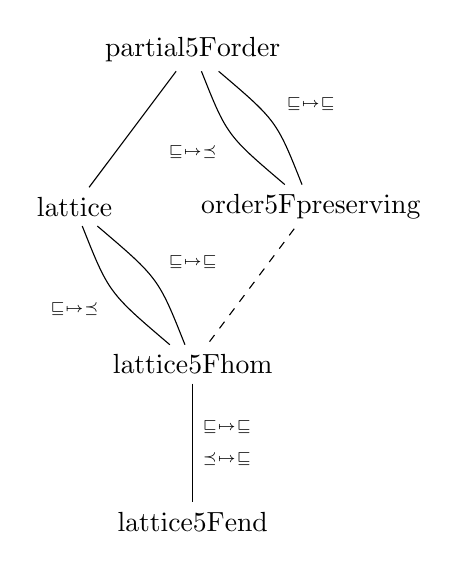
\begin{tikzpicture}
  \node (o) at (0,0) {\isa{partial{\isaliteral{5F}{\isacharunderscore}}order}};
  \node (oh) at (1.5,-2) {\isa{order{\isaliteral{5F}{\isacharunderscore}}preserving}};
  \node (oh1) at (1.5,-0.7) {$\scriptscriptstyle \sqsubseteq \mapsto \sqsubseteq$};
  \node (oh2) at (0,-1.3) {$\scriptscriptstyle \sqsubseteq \mapsto \preceq$};
  \node (l) at (-1.5,-2) {\isa{lattice}};
  \node (lh) at (0,-4) {\isa{lattice{\isaliteral{5F}{\isacharunderscore}}hom}};
  \node (lh1) at (0,-2.7) {$\scriptscriptstyle \sqsubseteq \mapsto \sqsubseteq$};
  \node (lh2) at (-1.5,-3.3) {$\scriptscriptstyle \sqsubseteq \mapsto \preceq$};
  \node (le) at (0,-6) {\isa{lattice{\isaliteral{5F}{\isacharunderscore}}end}};
  \node (le1) at (0,-4.8)
    [anchor=west]{$\scriptscriptstyle \sqsubseteq \mapsto \sqsubseteq$};
  \node (le2) at (0,-5.2)
    [anchor=west]{$\scriptscriptstyle \preceq \mapsto \sqsubseteq$};
  \draw (o) -- (l);
  \draw[dashed] (oh) -- (lh);
  \draw (lh) -- (le);
  \draw (o) .. controls (oh1.south west) .. (oh);
  \draw (o) .. controls (oh2.north east) .. (oh);
  \draw (l) .. controls (lh1.south west) .. (lh);
  \draw (l) .. controls (lh2.north east) .. (lh);
\end{tikzpicture}
\end{center}
\hrule
\caption{Hierarchy of Homomorphism Locales.}
\label{fig:hom}
\end{figure}%
\end{isamarkuptext}%
\isamarkuptrue%
%
\begin{isamarkuptext}%
It can be shown easily that a lattice homomorphism is order
  preserving.  As the final example of this section, a locale
  interpretation is used to assert this:%
\end{isamarkuptext}%
\isamarkuptrue%
\ \ \isacommand{sublocale}\isamarkupfalse%
\ lattice{\isaliteral{5F}{\isacharunderscore}}hom\ {\isaliteral{5C3C73756273657465713E}{\isasymsubseteq}}\ order{\isaliteral{5F}{\isacharunderscore}}preserving\isanewline
%
\isadelimproof
\ \ %
\endisadelimproof
%
\isatagproof
\isacommand{proof}\isamarkupfalse%
\ unfold{\isaliteral{5F}{\isacharunderscore}}locales\isanewline
\ \ \ \ \isacommand{fix}\isamarkupfalse%
\ x\ y\isanewline
\ \ \ \ \isacommand{assume}\isamarkupfalse%
\ {\isaliteral{22}{\isachardoublequoteopen}}x\ {\isaliteral{5C3C737173756273657465713E}{\isasymsqsubseteq}}\ y{\isaliteral{22}{\isachardoublequoteclose}}\isanewline
\ \ \ \ \isacommand{then}\isamarkupfalse%
\ \isacommand{have}\isamarkupfalse%
\ {\isaliteral{22}{\isachardoublequoteopen}}y\ {\isaliteral{3D}{\isacharequal}}\ {\isaliteral{28}{\isacharparenleft}}x\ {\isaliteral{5C3C7371756E696F6E3E}{\isasymsqunion}}\ y{\isaliteral{29}{\isacharparenright}}{\isaliteral{22}{\isachardoublequoteclose}}\ \isacommand{by}\isamarkupfalse%
\ {\isaliteral{28}{\isacharparenleft}}simp\ add{\isaliteral{3A}{\isacharcolon}}\ le{\isaliteral{2E}{\isachardot}}join{\isaliteral{5F}{\isacharunderscore}}connection{\isaliteral{29}{\isacharparenright}}\isanewline
\ \ \ \ \isacommand{then}\isamarkupfalse%
\ \isacommand{have}\isamarkupfalse%
\ {\isaliteral{22}{\isachardoublequoteopen}}{\isaliteral{5C3C7068693E}{\isasymphi}}\ y\ {\isaliteral{3D}{\isacharequal}}\ {\isaliteral{28}{\isacharparenleft}}{\isaliteral{5C3C7068693E}{\isasymphi}}\ x\ {\isaliteral{5C3C7371756E696F6E3E}{\isasymsqunion}}{\isaliteral{27}{\isacharprime}}\ {\isaliteral{5C3C7068693E}{\isasymphi}}\ y{\isaliteral{29}{\isacharparenright}}{\isaliteral{22}{\isachardoublequoteclose}}\ \isacommand{by}\isamarkupfalse%
\ {\isaliteral{28}{\isacharparenleft}}simp\ add{\isaliteral{3A}{\isacharcolon}}\ hom{\isaliteral{5F}{\isacharunderscore}}join\ {\isaliteral{5B}{\isacharbrackleft}}symmetric{\isaliteral{5D}{\isacharbrackright}}{\isaliteral{29}{\isacharparenright}}\isanewline
\ \ \ \ \isacommand{then}\isamarkupfalse%
\ \isacommand{show}\isamarkupfalse%
\ {\isaliteral{22}{\isachardoublequoteopen}}{\isaliteral{5C3C7068693E}{\isasymphi}}\ x\ {\isaliteral{5C3C7072656365713E}{\isasympreceq}}\ {\isaliteral{5C3C7068693E}{\isasymphi}}\ y{\isaliteral{22}{\isachardoublequoteclose}}\ \isacommand{by}\isamarkupfalse%
\ {\isaliteral{28}{\isacharparenleft}}simp\ add{\isaliteral{3A}{\isacharcolon}}\ le{\isaliteral{27}{\isacharprime}}{\isaliteral{2E}{\isachardot}}join{\isaliteral{5F}{\isacharunderscore}}connection{\isaliteral{29}{\isacharparenright}}\isanewline
\ \ \isacommand{qed}\isamarkupfalse%
%
\endisatagproof
{\isafoldproof}%
%
\isadelimproof
%
\endisadelimproof
%
\begin{isamarkuptext}%
Theorems and other declarations --- syntax, in particular --- from
  the locale \isa{order{\isaliteral{5F}{\isacharunderscore}}preserving} are now active in \isa{lattice{\isaliteral{5F}{\isacharunderscore}}hom}, for example
  \isa{hom{\isaliteral{5F}{\isacharunderscore}}le}:
  \begin{isabelle}%
\ \ {\isaliteral{3F}{\isacharquery}}x\ {\isaliteral{5C3C737173756273657465713E}{\isasymsqsubseteq}}\ {\isaliteral{3F}{\isacharquery}}y\ {\isaliteral{5C3C4C6F6E6772696768746172726F773E}{\isasymLongrightarrow}}\ {\isaliteral{5C3C7068693E}{\isasymphi}}\ {\isaliteral{3F}{\isacharquery}}x\ {\isaliteral{5C3C7072656365713E}{\isasympreceq}}\ {\isaliteral{5C3C7068693E}{\isasymphi}}\ {\isaliteral{3F}{\isacharquery}}y%
\end{isabelle}
  This theorem will be useful in the following section.%
\end{isamarkuptext}%
\isamarkuptrue%
%
\isamarkupsection{Conditional Interpretation%
}
\isamarkuptrue%
%
\begin{isamarkuptext}%
There are situations where an interpretation is not possible
  in the general case since the desired property is only valid if
  certain conditions are fulfilled.  Take, for example, the function
  \isa{{\isaliteral{5C3C6C616D6264613E}{\isasymlambda}}i{\isaliteral{2E}{\isachardot}}\ n\ {\isaliteral{2A}{\isacharasterisk}}\ i} that scales its argument by a constant factor.
  This function is order preserving (and even a lattice endomorphism)
  with respect to \isa{op\ {\isaliteral{5C3C6C653E}{\isasymle}}} provided \isa{n\ {\isaliteral{5C3C67653E}{\isasymge}}\ {\isadigit{0}}}.

  It is not possible to express this using a global interpretation,
  because it is in general unspecified whether~\isa{n} is
  non-negative, but one may make an interpretation in an inner context
  of a proof where full information is available.
  This is not fully satisfactory either, since potentially
  interpretations may be required to make interpretations in many
  contexts.  What is
  required is an interpretation that depends on the condition --- and
  this can be done with the \isakeyword{sublocale} command.  For this
  purpose, we introduce a locale for the condition.%
\end{isamarkuptext}%
\isamarkuptrue%
\ \ \isacommand{locale}\isamarkupfalse%
\ non{\isaliteral{5F}{\isacharunderscore}}negative\ {\isaliteral{3D}{\isacharequal}}\isanewline
\ \ \ \ \isakeyword{fixes}\ n\ {\isaliteral{3A}{\isacharcolon}}{\isaliteral{3A}{\isacharcolon}}\ int\isanewline
\ \ \ \ \isakeyword{assumes}\ non{\isaliteral{5F}{\isacharunderscore}}neg{\isaliteral{3A}{\isacharcolon}}\ {\isaliteral{22}{\isachardoublequoteopen}}{\isadigit{0}}\ {\isaliteral{5C3C6C653E}{\isasymle}}\ n{\isaliteral{22}{\isachardoublequoteclose}}%
\begin{isamarkuptext}%
It is again convenient to make the interpretation in an
  incremental fashion, first for order preserving maps, the for
  lattice endomorphisms.%
\end{isamarkuptext}%
\isamarkuptrue%
\ \ \isacommand{sublocale}\isamarkupfalse%
\ non{\isaliteral{5F}{\isacharunderscore}}negative\ {\isaliteral{5C3C73756273657465713E}{\isasymsubseteq}}\isanewline
\ \ \ \ \ \ order{\isaliteral{5F}{\isacharunderscore}}preserving\ {\isaliteral{22}{\isachardoublequoteopen}}op\ {\isaliteral{5C3C6C653E}{\isasymle}}{\isaliteral{22}{\isachardoublequoteclose}}\ {\isaliteral{22}{\isachardoublequoteopen}}op\ {\isaliteral{5C3C6C653E}{\isasymle}}{\isaliteral{22}{\isachardoublequoteclose}}\ {\isaliteral{22}{\isachardoublequoteopen}}{\isaliteral{5C3C6C616D6264613E}{\isasymlambda}}i{\isaliteral{2E}{\isachardot}}\ n\ {\isaliteral{2A}{\isacharasterisk}}\ i{\isaliteral{22}{\isachardoublequoteclose}}\isanewline
%
\isadelimproof
\ \ \ \ %
\endisadelimproof
%
\isatagproof
\isacommand{using}\isamarkupfalse%
\ non{\isaliteral{5F}{\isacharunderscore}}neg\ \isacommand{by}\isamarkupfalse%
\ unfold{\isaliteral{5F}{\isacharunderscore}}locales\ {\isaliteral{28}{\isacharparenleft}}rule\ mult{\isaliteral{5F}{\isacharunderscore}}left{\isaliteral{5F}{\isacharunderscore}}mono{\isaliteral{29}{\isacharparenright}}%
\endisatagproof
{\isafoldproof}%
%
\isadelimproof
%
\endisadelimproof
%
\begin{isamarkuptext}%
While the proof of the previous interpretation
  is straightforward from monotonicity lemmas for~\isa{op\ {\isaliteral{2A}{\isacharasterisk}}}, the
  second proof follows a useful pattern.%
\end{isamarkuptext}%
\isamarkuptrue%
%
\isadelimvisible
\ \ %
\endisadelimvisible
%
\isatagvisible
\isacommand{sublocale}\isamarkupfalse%
\ non{\isaliteral{5F}{\isacharunderscore}}negative\ {\isaliteral{5C3C73756273657465713E}{\isasymsubseteq}}\ lattice{\isaliteral{5F}{\isacharunderscore}}end\ {\isaliteral{22}{\isachardoublequoteopen}}op\ {\isaliteral{5C3C6C653E}{\isasymle}}{\isaliteral{22}{\isachardoublequoteclose}}\ {\isaliteral{22}{\isachardoublequoteopen}}{\isaliteral{5C3C6C616D6264613E}{\isasymlambda}}i{\isaliteral{2E}{\isachardot}}\ n\ {\isaliteral{2A}{\isacharasterisk}}\ i{\isaliteral{22}{\isachardoublequoteclose}}\isanewline
\ \ \isacommand{proof}\isamarkupfalse%
\ {\isaliteral{28}{\isacharparenleft}}unfold{\isaliteral{5F}{\isacharunderscore}}locales{\isaliteral{2C}{\isacharcomma}}\ unfold\ int{\isaliteral{5F}{\isacharunderscore}}min{\isaliteral{5F}{\isacharunderscore}}eq\ int{\isaliteral{5F}{\isacharunderscore}}max{\isaliteral{5F}{\isacharunderscore}}eq{\isaliteral{29}{\isacharparenright}}%
\begin{isamarkuptxt}%
\normalsize Unfolding the locale predicates \emph{and} the
      interpretation equations immediately yields two subgoals that
      reflect the core conjecture.
      \begin{isabelle}%
\ {\isadigit{1}}{\isaliteral{2E}{\isachardot}}\ {\isaliteral{5C3C416E643E}{\isasymAnd}}x\ y{\isaliteral{2E}{\isachardot}}\ n\ {\isaliteral{2A}{\isacharasterisk}}\ min\ x\ y\ {\isaliteral{3D}{\isacharequal}}\ min\ {\isaliteral{28}{\isacharparenleft}}n\ {\isaliteral{2A}{\isacharasterisk}}\ x{\isaliteral{29}{\isacharparenright}}\ {\isaliteral{28}{\isacharparenleft}}n\ {\isaliteral{2A}{\isacharasterisk}}\ y{\isaliteral{29}{\isacharparenright}}\isanewline
\ {\isadigit{2}}{\isaliteral{2E}{\isachardot}}\ {\isaliteral{5C3C416E643E}{\isasymAnd}}x\ y{\isaliteral{2E}{\isachardot}}\ n\ {\isaliteral{2A}{\isacharasterisk}}\ max\ x\ y\ {\isaliteral{3D}{\isacharequal}}\ max\ {\isaliteral{28}{\isacharparenleft}}n\ {\isaliteral{2A}{\isacharasterisk}}\ x{\isaliteral{29}{\isacharparenright}}\ {\isaliteral{28}{\isacharparenleft}}n\ {\isaliteral{2A}{\isacharasterisk}}\ y{\isaliteral{29}{\isacharparenright}}%
\end{isabelle}
      It is now necessary to show, in the context of \isa{non{\isaliteral{5F}{\isacharunderscore}}negative}, that multiplication by~\isa{n} commutes with
      \isa{min} and \isa{max}.%
\end{isamarkuptxt}%
\isamarkuptrue%
\ \ \isacommand{qed}\isamarkupfalse%
\ {\isaliteral{28}{\isacharparenleft}}auto\ simp{\isaliteral{3A}{\isacharcolon}}\ hom{\isaliteral{5F}{\isacharunderscore}}le{\isaliteral{29}{\isacharparenright}}%
\endisatagvisible
{\isafoldvisible}%
%
\isadelimvisible
%
\endisadelimvisible
%
\begin{isamarkuptext}%
The lemma \isa{hom{\isaliteral{5F}{\isacharunderscore}}le}
  simplifies a proof that would have otherwise been lengthy and we may
  consider making it a default rule for the simplifier:%
\end{isamarkuptext}%
\isamarkuptrue%
\ \ \isacommand{lemmas}\isamarkupfalse%
\ {\isaliteral{28}{\isacharparenleft}}\isakeyword{in}\ order{\isaliteral{5F}{\isacharunderscore}}preserving{\isaliteral{29}{\isacharparenright}}\ hom{\isaliteral{5F}{\isacharunderscore}}le\ {\isaliteral{5B}{\isacharbrackleft}}simp{\isaliteral{5D}{\isacharbrackright}}%
\isamarkupsubsection{Avoiding Infinite Chains of Interpretations
  \label{sec:infinite-chains}%
}
\isamarkuptrue%
%
\begin{isamarkuptext}%
Similar situations arise frequently in formalisations of
  abstract algebra where it is desirable to express that certain
  constructions preserve certain properties.  For example, polynomials
  over rings are rings, or --- an example from the domain where the
  illustrations of this tutorial are taken from --- a partial order
  may be obtained for a function space by point-wise lifting of the
  partial order of the co-domain.  This corresponds to the following
  interpretation:%
\end{isamarkuptext}%
\isamarkuptrue%
%
\isadelimvisible
\ \ %
\endisadelimvisible
%
\isatagvisible
\isacommand{sublocale}\isamarkupfalse%
\ partial{\isaliteral{5F}{\isacharunderscore}}order\ {\isaliteral{5C3C73756273657465713E}{\isasymsubseteq}}\ f{\isaliteral{3A}{\isacharcolon}}\ partial{\isaliteral{5F}{\isacharunderscore}}order\ {\isaliteral{22}{\isachardoublequoteopen}}{\isaliteral{5C3C6C616D6264613E}{\isasymlambda}}f\ g{\isaliteral{2E}{\isachardot}}\ {\isaliteral{5C3C666F72616C6C3E}{\isasymforall}}x{\isaliteral{2E}{\isachardot}}\ f\ x\ {\isaliteral{5C3C737173756273657465713E}{\isasymsqsubseteq}}\ g\ x{\isaliteral{22}{\isachardoublequoteclose}}\isanewline
\ \ \ \ \isacommand{oops}\isamarkupfalse%
%
\endisatagvisible
{\isafoldvisible}%
%
\isadelimvisible
%
\endisadelimvisible
%
\begin{isamarkuptext}%
Unfortunately this is a cyclic interpretation that leads to an
  infinite chain, namely
  \begin{isabelle}%
\ \ partial{\isaliteral{5F}{\isacharunderscore}}order\ {\isaliteral{5C3C73756273657465713E}{\isasymsubseteq}}\ partial{\isaliteral{5F}{\isacharunderscore}}order\ {\isaliteral{28}{\isacharparenleft}}{\isaliteral{5C3C6C616D6264613E}{\isasymlambda}}f\ g{\isaliteral{2E}{\isachardot}}\ {\isaliteral{5C3C666F72616C6C3E}{\isasymforall}}x{\isaliteral{2E}{\isachardot}}\ f\ x\ {\isaliteral{5C3C737173756273657465713E}{\isasymsqsubseteq}}\ g\ x{\isaliteral{29}{\isacharparenright}}\ {\isaliteral{5C3C73756273657465713E}{\isasymsubseteq}}\isanewline
\isaindent{\ \ }\ \ partial{\isaliteral{5F}{\isacharunderscore}}order\ {\isaliteral{28}{\isacharparenleft}}{\isaliteral{5C3C6C616D6264613E}{\isasymlambda}}f\ g{\isaliteral{2E}{\isachardot}}\ {\isaliteral{5C3C666F72616C6C3E}{\isasymforall}}x\ y{\isaliteral{2E}{\isachardot}}\ f\ x\ y\ {\isaliteral{5C3C737173756273657465713E}{\isasymsqsubseteq}}\ g\ x\ y{\isaliteral{29}{\isacharparenright}}\ {\isaliteral{5C3C73756273657465713E}{\isasymsubseteq}}\ \ {\isaliteral{5C3C646F74733E}{\isasymdots}}%
\end{isabelle}
  and the interpretation is rejected.

  Instead it is necessary to declare a locale that is logically
  equivalent to \isa{partial{\isaliteral{5F}{\isacharunderscore}}order} but serves to collect facts
  about functions spaces where the co-domain is a partial order, and
  to make the interpretation in its context:%
\end{isamarkuptext}%
\isamarkuptrue%
\ \ \isacommand{locale}\isamarkupfalse%
\ fun{\isaliteral{5F}{\isacharunderscore}}partial{\isaliteral{5F}{\isacharunderscore}}order\ {\isaliteral{3D}{\isacharequal}}\ partial{\isaliteral{5F}{\isacharunderscore}}order\isanewline
\isanewline
\ \ \isacommand{sublocale}\isamarkupfalse%
\ fun{\isaliteral{5F}{\isacharunderscore}}partial{\isaliteral{5F}{\isacharunderscore}}order\ {\isaliteral{5C3C73756273657465713E}{\isasymsubseteq}}\isanewline
\ \ \ \ \ \ f{\isaliteral{3A}{\isacharcolon}}\ partial{\isaliteral{5F}{\isacharunderscore}}order\ {\isaliteral{22}{\isachardoublequoteopen}}{\isaliteral{5C3C6C616D6264613E}{\isasymlambda}}f\ g{\isaliteral{2E}{\isachardot}}\ {\isaliteral{5C3C666F72616C6C3E}{\isasymforall}}x{\isaliteral{2E}{\isachardot}}\ f\ x\ {\isaliteral{5C3C737173756273657465713E}{\isasymsqsubseteq}}\ g\ x{\isaliteral{22}{\isachardoublequoteclose}}\isanewline
%
\isadelimproof
\ \ \ \ %
\endisadelimproof
%
\isatagproof
\isacommand{by}\isamarkupfalse%
\ unfold{\isaliteral{5F}{\isacharunderscore}}locales\ {\isaliteral{28}{\isacharparenleft}}fast{\isaliteral{2C}{\isacharcomma}}rule{\isaliteral{2C}{\isacharcomma}}fast{\isaliteral{2C}{\isacharcomma}}blast\ intro{\isaliteral{3A}{\isacharcolon}}\ trans{\isaliteral{29}{\isacharparenright}}%
\endisatagproof
{\isafoldproof}%
%
\isadelimproof
%
\endisadelimproof
%
\begin{isamarkuptext}%
It is quite common in abstract algebra that such a construction
  maps a hierarchy of algebraic structures (or specifications) to a
  related hierarchy.  By means of the same lifting, a function space
  is a lattice if its co-domain is a lattice:%
\end{isamarkuptext}%
\isamarkuptrue%
\ \ \isacommand{locale}\isamarkupfalse%
\ fun{\isaliteral{5F}{\isacharunderscore}}lattice\ {\isaliteral{3D}{\isacharequal}}\ fun{\isaliteral{5F}{\isacharunderscore}}partial{\isaliteral{5F}{\isacharunderscore}}order\ {\isaliteral{2B}{\isacharplus}}\ lattice\isanewline
\isanewline
\ \ \isacommand{sublocale}\isamarkupfalse%
\ fun{\isaliteral{5F}{\isacharunderscore}}lattice\ {\isaliteral{5C3C73756273657465713E}{\isasymsubseteq}}\ f{\isaliteral{3A}{\isacharcolon}}\ lattice\ {\isaliteral{22}{\isachardoublequoteopen}}{\isaliteral{5C3C6C616D6264613E}{\isasymlambda}}f\ g{\isaliteral{2E}{\isachardot}}\ {\isaliteral{5C3C666F72616C6C3E}{\isasymforall}}x{\isaliteral{2E}{\isachardot}}\ f\ x\ {\isaliteral{5C3C737173756273657465713E}{\isasymsqsubseteq}}\ g\ x{\isaliteral{22}{\isachardoublequoteclose}}\isanewline
%
\isadelimproof
\ \ %
\endisadelimproof
%
\isatagproof
\isacommand{proof}\isamarkupfalse%
\ unfold{\isaliteral{5F}{\isacharunderscore}}locales\isanewline
\ \ \ \ \isacommand{fix}\isamarkupfalse%
\ f\ g\isanewline
\ \ \ \ \isacommand{have}\isamarkupfalse%
\ {\isaliteral{22}{\isachardoublequoteopen}}partial{\isaliteral{5F}{\isacharunderscore}}order{\isaliteral{2E}{\isachardot}}is{\isaliteral{5F}{\isacharunderscore}}inf\ {\isaliteral{28}{\isacharparenleft}}{\isaliteral{5C3C6C616D6264613E}{\isasymlambda}}f\ g{\isaliteral{2E}{\isachardot}}\ {\isaliteral{5C3C666F72616C6C3E}{\isasymforall}}x{\isaliteral{2E}{\isachardot}}\ f\ x\ {\isaliteral{5C3C737173756273657465713E}{\isasymsqsubseteq}}\ g\ x{\isaliteral{29}{\isacharparenright}}\ f\ g\ {\isaliteral{28}{\isacharparenleft}}{\isaliteral{5C3C6C616D6264613E}{\isasymlambda}}x{\isaliteral{2E}{\isachardot}}\ f\ x\ {\isaliteral{5C3C7371696E7465723E}{\isasymsqinter}}\ g\ x{\isaliteral{29}{\isacharparenright}}{\isaliteral{22}{\isachardoublequoteclose}}\isanewline
\ \ \ \ \ \ \isacommand{apply}\isamarkupfalse%
\ {\isaliteral{28}{\isacharparenleft}}rule\ is{\isaliteral{5F}{\isacharunderscore}}infI{\isaliteral{29}{\isacharparenright}}\ \isacommand{apply}\isamarkupfalse%
\ rule{\isaliteral{2B}{\isacharplus}}\ \isacommand{apply}\isamarkupfalse%
\ {\isaliteral{28}{\isacharparenleft}}drule\ spec{\isaliteral{2C}{\isacharcomma}}\ assumption{\isaliteral{29}{\isacharparenright}}{\isaliteral{2B}{\isacharplus}}\ \isacommand{done}\isamarkupfalse%
\isanewline
\ \ \ \ \isacommand{then}\isamarkupfalse%
\ \isacommand{show}\isamarkupfalse%
\ {\isaliteral{22}{\isachardoublequoteopen}}{\isaliteral{5C3C6578697374733E}{\isasymexists}}inf{\isaliteral{2E}{\isachardot}}\ partial{\isaliteral{5F}{\isacharunderscore}}order{\isaliteral{2E}{\isachardot}}is{\isaliteral{5F}{\isacharunderscore}}inf\ {\isaliteral{28}{\isacharparenleft}}{\isaliteral{5C3C6C616D6264613E}{\isasymlambda}}f\ g{\isaliteral{2E}{\isachardot}}\ {\isaliteral{5C3C666F72616C6C3E}{\isasymforall}}x{\isaliteral{2E}{\isachardot}}\ f\ x\ {\isaliteral{5C3C737173756273657465713E}{\isasymsqsubseteq}}\ g\ x{\isaliteral{29}{\isacharparenright}}\ f\ g\ inf{\isaliteral{22}{\isachardoublequoteclose}}\isanewline
\ \ \ \ \ \ \isacommand{by}\isamarkupfalse%
\ fast\isanewline
\ \ \isacommand{next}\isamarkupfalse%
\isanewline
\ \ \ \ \isacommand{fix}\isamarkupfalse%
\ f\ g\isanewline
\ \ \ \ \isacommand{have}\isamarkupfalse%
\ {\isaliteral{22}{\isachardoublequoteopen}}partial{\isaliteral{5F}{\isacharunderscore}}order{\isaliteral{2E}{\isachardot}}is{\isaliteral{5F}{\isacharunderscore}}sup\ {\isaliteral{28}{\isacharparenleft}}{\isaliteral{5C3C6C616D6264613E}{\isasymlambda}}f\ g{\isaliteral{2E}{\isachardot}}\ {\isaliteral{5C3C666F72616C6C3E}{\isasymforall}}x{\isaliteral{2E}{\isachardot}}\ f\ x\ {\isaliteral{5C3C737173756273657465713E}{\isasymsqsubseteq}}\ g\ x{\isaliteral{29}{\isacharparenright}}\ f\ g\ {\isaliteral{28}{\isacharparenleft}}{\isaliteral{5C3C6C616D6264613E}{\isasymlambda}}x{\isaliteral{2E}{\isachardot}}\ f\ x\ {\isaliteral{5C3C7371756E696F6E3E}{\isasymsqunion}}\ g\ x{\isaliteral{29}{\isacharparenright}}{\isaliteral{22}{\isachardoublequoteclose}}\isanewline
\ \ \ \ \ \ \isacommand{apply}\isamarkupfalse%
\ {\isaliteral{28}{\isacharparenleft}}rule\ is{\isaliteral{5F}{\isacharunderscore}}supI{\isaliteral{29}{\isacharparenright}}\ \isacommand{apply}\isamarkupfalse%
\ rule{\isaliteral{2B}{\isacharplus}}\ \isacommand{apply}\isamarkupfalse%
\ {\isaliteral{28}{\isacharparenleft}}drule\ spec{\isaliteral{2C}{\isacharcomma}}\ assumption{\isaliteral{29}{\isacharparenright}}{\isaliteral{2B}{\isacharplus}}\ \isacommand{done}\isamarkupfalse%
\isanewline
\ \ \ \ \isacommand{then}\isamarkupfalse%
\ \isacommand{show}\isamarkupfalse%
\ {\isaliteral{22}{\isachardoublequoteopen}}{\isaliteral{5C3C6578697374733E}{\isasymexists}}sup{\isaliteral{2E}{\isachardot}}\ partial{\isaliteral{5F}{\isacharunderscore}}order{\isaliteral{2E}{\isachardot}}is{\isaliteral{5F}{\isacharunderscore}}sup\ {\isaliteral{28}{\isacharparenleft}}{\isaliteral{5C3C6C616D6264613E}{\isasymlambda}}f\ g{\isaliteral{2E}{\isachardot}}\ {\isaliteral{5C3C666F72616C6C3E}{\isasymforall}}x{\isaliteral{2E}{\isachardot}}\ f\ x\ {\isaliteral{5C3C737173756273657465713E}{\isasymsqsubseteq}}\ g\ x{\isaliteral{29}{\isacharparenright}}\ f\ g\ sup{\isaliteral{22}{\isachardoublequoteclose}}\isanewline
\ \ \ \ \ \ \isacommand{by}\isamarkupfalse%
\ fast\isanewline
\ \ \isacommand{qed}\isamarkupfalse%
%
\endisatagproof
{\isafoldproof}%
%
\isadelimproof
%
\endisadelimproof
%
\isamarkupsection{Further Reading%
}
\isamarkuptrue%
%
\begin{isamarkuptext}%
More information on locales and their interpretation is
  available.  For the locale hierarchy of import and interpretation
  dependencies see~\cite{Ballarin2006a}; interpretations in theories
  and proofs are covered in~\cite{Ballarin2006b}.  In the latter, I
  show how interpretation in proofs enables to reason about families
  of algebraic structures, which cannot be expressed with locales
  directly.

  Haftmann and Wenzel~\cite{HaftmannWenzel2007} overcome a restriction
  of axiomatic type classes through a combination with locale
  interpretation.  The result is a Haskell-style class system with a
  facility to generate ML and Haskell code.  Classes are sufficient for
  simple specifications with a single type parameter.  The locales for
  orders and lattices presented in this tutorial fall into this
  category.  Order preserving maps, homomorphisms and vector spaces,
  on the other hand, do not.

  The locales reimplementation for Isabelle 2009 provides, among other
  improvements, a clean integration with Isabelle/Isar's local theory
  mechanisms, which are described in another paper by Haftmann and
  Wenzel~\cite{HaftmannWenzel2009}.

  The original work of Kamm\"uller on locales~\cite{KammullerEtAl1999}
  may be of interest from a historical perspective.  My previous
  report on locales and locale expressions~\cite{Ballarin2004a}
  describes a simpler form of expressions than available now and is
  outdated. The mathematical background on orders and lattices is
  taken from Jacobson's textbook on algebra~\cite[Chapter~8]{Jacobson1985}.

  The sources of this tutorial, which include all proofs, are
  available with the Isabelle distribution at
  \url{http://isabelle.in.tum.de}.%
\end{isamarkuptext}%
\isamarkuptrue%
%
\begin{isamarkuptext}%
\begin{table}
\hrule
\vspace{2ex}
\begin{center}
\begin{tabular}{l>$c<$l}
  \multicolumn{3}{l}{Miscellaneous} \\

  \textit{attr-name} & ::=
  & \textit{name} $|$ \textit{attribute} $|$
    \textit{name} \textit{attribute} \\
  \textit{qualifier} & ::=
  & \textit{name} [``\textbf{?}'' $|$ ``\textbf{!}''] \\[2ex]

  \multicolumn{3}{l}{Context Elements} \\

  \textit{fixes} & ::=
  & \textit{name} [ ``\textbf{::}'' \textit{type} ]
    [ ``\textbf{(}'' \textbf{structure} ``\textbf{)}'' $|$
    \textit{mixfix} ] \\
\begin{comment}
  \textit{constrains} & ::=
  & \textit{name} ``\textbf{::}'' \textit{type} \\
\end{comment}
  \textit{assumes} & ::=
  & [ \textit{attr-name} ``\textbf{:}'' ] \textit{proposition} \\
\begin{comment}
  \textit{defines} & ::=
  & [ \textit{attr-name} ``\textbf{:}'' ] \textit{proposition} \\
  \textit{notes} & ::=
  & [ \textit{attr-name} ``\textbf{=}'' ]
    ( \textit{qualified-name} [ \textit{attribute} ] )$^+$ \\
\end{comment}

  \textit{element} & ::=
  & \textbf{fixes} \textit{fixes} ( \textbf{and} \textit{fixes} )$^*$ \\
\begin{comment}
  & |
  & \textbf{constrains} \textit{constrains}
    ( \textbf{and} \textit{constrains} )$^*$ \\
\end{comment}
  & |
  & \textbf{assumes} \textit{assumes} ( \textbf{and} \textit{assumes} )$^*$ \\[2ex]
%\begin{comment}
%  & |
%  & \textbf{defines} \textit{defines} ( \textbf{and} \textit{defines} )$^*$ \\
%  & |
%  & \textbf{notes} \textit{notes} ( \textbf{and} \textit{notes} )$^*$ \\
%\end{comment}

  \multicolumn{3}{l}{Locale Expressions} \\

  \textit{pos-insts} & ::=
  & ( \textit{term} $|$ ``\textbf{\_}'' )$^*$ \\
  \textit{named-insts} & ::=
  & \textbf{where} \textit{name} ``\textbf{=}'' \textit{term}
  ( \textbf{and} \textit{name} ``\textbf{=}'' \textit{term} )$^*$ \\
  \textit{instance} & ::=
  & [ \textit{qualifier} ``\textbf{:}'' ]
    \textit{name} ( \textit{pos-insts} $|$ \textit{named-inst} ) \\
  \textit{expression}  & ::= 
  & \textit{instance} ( ``\textbf{+}'' \textit{instance} )$^*$
    [ \textbf{for} \textit{fixes} ( \textbf{and} \textit{fixes} )$^*$ ] \\[2ex]

  \multicolumn{3}{l}{Declaration of Locales} \\

  \textit{locale} & ::=
  & \textit{element}$^+$ \\
  & | & \textit{expression} [ ``\textbf{+}'' \textit{element}$^+$ ] \\
  \textit{toplevel} & ::=
  & \textbf{locale} \textit{name} [ ``\textbf{=}''
    \textit{locale} ] \\[2ex]

  \multicolumn{3}{l}{Interpretation} \\

  \textit{equation} & ::= & [ \textit{attr-name} ``\textbf{:}'' ]
    \textit{prop} \\
  \textit{equations} & ::= &  \textbf{where} \textit{equation} ( \textbf{and}
    \textit{equation} )$^*$  \\
  \textit{toplevel} & ::=
  & \textbf{sublocale} \textit{name} ( ``$<$'' $|$
    ``$\subseteq$'' ) \textit{expression} \textit{proof} \\
  & |
  & \textbf{interpretation}
    \textit{expression} [ \textit{equations} ] \textit{proof} \\
  & |
  & \textbf{interpret}
    \textit{expression} \textit{proof} \\[2ex]

  \multicolumn{3}{l}{Diagnostics} \\

  \textit{toplevel} & ::=
  & \textbf{print\_locales} \\
  & | & \textbf{print\_locale} [ ``\textbf{!}'' ] \textit{name} \\
  & | & \textbf{print\_interps} \textit{name}
\end{tabular}
\end{center}
\hrule
\caption{Syntax of Locale Commands.}
\label{tab:commands}
\end{table}%
\end{isamarkuptext}%
\isamarkuptrue%
%
\begin{isamarkuptext}%
\textbf{Revision History.}  For the present third revision of
  the tutorial, much of the explanatory text
  was rewritten.  Inheritance of interpretation equations is
  available with the forthcoming release of Isabelle, which at the
  time of editing these notes is expected for the end of 2009.
  The second revision accommodates changes introduced by the locales
  reimplementation for Isabelle 2009.  Most notably locale expressions
  have been generalised from renaming to instantiation.%
\end{isamarkuptext}%
\isamarkuptrue%
%
\begin{isamarkuptext}%
\textbf{Acknowledgements.}  Alexander Krauss, Tobias Nipkow,
  Randy Pollack, Andreas Schropp, Christian Sternagel and Makarius Wenzel
  have made
  useful comments on earlier versions of this document.  The section
  on conditional interpretation was inspired by a number of e-mail
  enquiries the author received from locale users, and which suggested
  that this use case is important enough to deserve explicit
  explanation.  The term \emph{conditional interpretation} is due to
  Larry Paulson.%
\end{isamarkuptext}%
\isamarkuptrue%
%
\isadelimtheory
%
\endisadelimtheory
%
\isatagtheory
\isacommand{end}\isamarkupfalse%
%
\endisatagtheory
{\isafoldtheory}%
%
\isadelimtheory
%
\endisadelimtheory
\isanewline
\end{isabellebody}%
%%% Local Variables:
%%% mode: latex
%%% TeX-master: "root"
%%% End:
